\RequirePackage[l2tabu, orthodox]{nag}
\documentclass[a4paper, twocolumn]{article}
\usepackage[utf8]{inputenc}
\usepackage[T1]{fontenc}
\usepackage[pdftex, hidelinks,
            pdftitle={Behaviour Tree Evolution by Genetic Programming},
            pdfauthor={Martin Estgren and Erik S. V. Jansson},
            pdfsubject={Artificial Intelligence - Genetic Programming},
            pdfkeywords={artificial intelligence, genetic programming,
                         behaviour trees, a-star, shooter}]{hyperref}

\usepackage{bm}
\usepackage{caption}
\usepackage{listings}
\usepackage{booktabs}
\usepackage{mathtools}
\usepackage{algorithmic}
\usepackage{graphicx}
\usepackage{courier}
\usepackage{amsmath}
\usepackage{amssymb}
\usepackage{algorithm}
\usepackage[capitalize, noabbrev]{cleveref}
\usepackage[activate={true, nocompatibility}, final,
            tracking=true, kerning=true, spacing=true,
            factor=1100, stretch=10, shrink=10]{microtype}

\DeclareCaptionFormat{modifiedlst}{\rule{\textwidth}{0.85pt}\\[-2.9pt]#1#2#3}
\captionsetup[lstlisting]{format =  modifiedlst,
labelfont=bf,singlelinecheck=off,labelsep=space}
\lstset{basicstyle=\footnotesize\ttfamily,
        breakatwhitespace = false,
        breaklines = true,
        keepspaces = true,
        language = Java,
        showspaces = false,
        showstringspaces = false,
        frame = tb,
        numbers = left,
        numbersep = 5pt,
        xleftmargin = 16pt,
        framexleftmargin = 16pt,
        belowskip = \bigskipamount,
        aboveskip = \bigskipamount,
        escapeinside={<@}{@>}}

\title{\textbf{Behaviour Tree Evolution by Genetic Programming}\\
       \Large{\emph{-- Learning Novel Bot Behaviours in a 2D Top-Down Arena Shooter --}}}
\author{{\textbf{Martin Estgren}} \;\;\;\;\;\;\;\;\;\, {\href{mailto:mares480@student.liu.se}
                                                       {\texttt{<mares480@student.liu.se>}}} \\
        {\textbf{Erik S. V. Jansson}} \;\;\;\;         {\href{mailto:erija578@student.liu.se}
                                                       {\texttt{<erija578@student.liu.se>}}} \\~\\
        {Linköping University, Sweden}\vspace{-2.0ex}}

\begin{document}
    \maketitle
    \section*{Abstract}

    Behaviour trees are a popular model for representing the decision-making and plan execution process for NPCs in video games. These are built by hand, and require expertise to craft. They don't adapt well to other environments, and often require a custom BT.

    In this paper we demonstrate how to generate the BTs by using genetic programming; allowing us to essentially evolve novel behaviours automatically in our testbed. Results show that the evolved BT beats our hand-crafted BT by the \(5^{th}\) generation. \footnote{Repository: \url{https://github.com/sci10n/Quake2D}}

    \vspace{2.4em}

    \begingroup
    \def\addvspace#1{}
    \tableofcontents
    \endgroup
    \newpage

    \newpage % Next column...
    \nocite{*} % Include all.
    \bibliographystyle{abbrv}
    \bibliography{report}
    \clearpage

    \section{Introduction} \label{sec:introduction}

    In interactive media such as games, there is often a need for simulating seemingly complex agent behaviors in real-time. In modern fast-paced computer games for example, the render, physics and artificial intelligence steps all need to complete in a total of less than 16ms to provide a half-decent experience. These requirements have spawned some clever techniques to enable complex behaviors for autonomous agents, while keeping their computation time short.

    These techniques often require manual behaviour definition, and in some cases, are hard to extend when new behaviors are needed for a game, as shown by industry researchers, e.g. \emph{Dawe et al}~\cite{dawe2014overview}, regarding the finite state machine architecture. In this project we have explored how one of the more widely used techniques, \emph{behavior trees}, can be extended to allow for not only hand-crafted complex behaviors, but for organic behaviors tailored to the specific game domain by using \emph{reinforcement learning}. More specifically, we evolve behaviour trees with \emph{genetic programming}, which spawn behaviour tree offspring.

    Alongside the proposed method in \cref{sec:proposed_approach}, a testbed consisting of a top-down arena shooter was built. It features a sufficiently complex environment to support interesting behaviours by the enemy bot. We describe the features of our testbed in \cref{sec:implementation_details}.

    This report starts off in \cref{sec:background_theory} by giving a brief overview of the relevant techniques and related work necessary to follow our reasoning and findings. In \cref{sec:implementation_details} we describe the details needed to implement these techniques in practice, along with the testbed architecture we've used. This gives the reader information on any peculiarities and pit-falls. We follow this by showing in \cref{sec:results_and_screenshots} the testbed, and give some generated offspring generated by our method along with measurements of its efficiency. Finally, we reflect on our method, giving downsides, and present some possible future work in \cref{sec:discussion_and_outlook}.

    \vspace{-0.8em}

    \subsection{Proposed Approach} \label{sec:proposed_approach}

    Apply \emph{genetic programming} to the \emph{behaviours trees} by creating \emph{high-level actions and conditions} nodes. Ideally this should allow for faster convergence rates and somewhat shallower generated behaviour trees, eliminating the need for bloat control and pruning. Since BTs are trees, the \emph{mutation mechanism} should modify \emph{control-flow structure} and \emph{leaf-node settings}, while the \emph{crossover mechanism} will swap sub-trees.

    \section{Background Theory} \label{sec:background_theory}

    For a autonomous agent to give the illusion of intelligence, many different systems need to interact. In the case of this project, the spatial path-finding and the behavior model has been decoupled where the path-finding system only receives a target position in the simulated environment and left to find the best path to the target by it self.

        \subsection{Behaviour Trees} \label{sec:behaviour_trees}

        \begin{figure}[H]
            \centering
            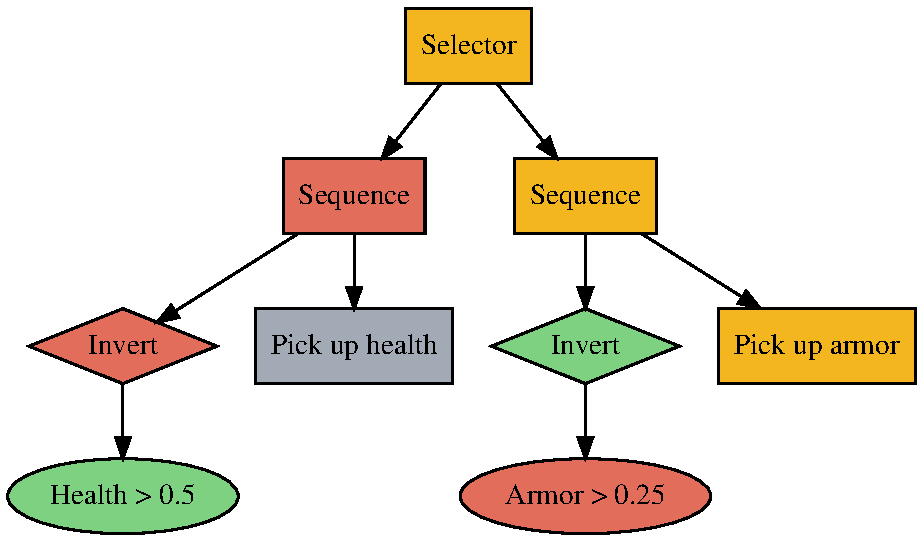
\includegraphics[width=\linewidth]{share/behaviour_tree.pdf}
            \caption{Example of Hand-Crafted Behaviour Tree}
            \label{fig:behaviour_tree}
        \end{figure}

        \subsection{Path Finding with A*} \label{sec:path_finding}

	Agent path finding is done using the \emph{A*} graph traversal algorithm propsed by Peter E. Hart, Nils J. Nilsson, and Bertram Raphael ~\cite{hart1968formal} as an extension to \emph{Dijkstra's algorithm} which, given an \emph{admissible heuristic} and non-negative costs, will find the path from a node \(s\) to node \(n\) with the lowest cost.
	

        \subsection{Genetic Programming} \label{sec:genetic_programming}



    \section{Implementation Details} \label{sec:implementation_details}



        \subsection{Game Architecture} \label{sec:game_architecture}



        \subsection{Behaviour Trees} \label{sec:behaviour_trees_implementation}



        \subsection{Path Finding with A*} \label{sec:path_finding_implementation}



        \subsection{Genetic Programming} \label{sec:genetic_programming_implementation}



    \section{Results and Screenshots} \label{sec:results_and_screenshots}



        \subsection{Generated Behaviours} \label{sec:generated_behaviours}



        \subsection{Behaviour Fitness} \label{sec:behaviour_fitness}



        \subsection{Survival Rate} \label{sec:survival_rate}



    \section{Discussion and Outlook} \label{sec:discussion_and_outlook}



\end{document}
